% !TeX spellcheck = en
\documentclass{article}
\usepackage{float}
\usepackage{graphicx}
\usepackage{hyperref}
\usepackage[utf8]{inputenc}
\usepackage{pdfpages}

\author{Mikael Lindemann Jepsen}
\date{\today}
\title{Measurements of naive matrix multiplication}

\begin{document}
	\maketitle
	\section{Intro}
	\begin{description}
		\item [The Problem] Measurement of naive matrix multiplication in different programming languages.
		\item [Languages] I have chosen to implement the naive matrix multiplication in C and Java. Furthermore there is a threaded implementation of the Java code.
	\end{description}

	\section{Methods}
	\begin{description}
		\item[System] The programs are run on Ubuntu 16.04 provided by the ITU.
		\item[Compiler] The C compiler used is GCC 5.4.0 with the -O2 optimization flags enabled. OpenJDK version 8 is used for the Java implementations.
		\item[Fetures used] The C program is single threaded. One Java implementation is single threaded, and another is multi-threaded. It should be straight forward to implement a threaded C edition by use of Pthreads, but I did not have the time for it.
		\item[Measurement] The time of the programs are timed using the Debian/GNU Linux \texttt{time} command. The time measured is the \textit{real}/wall clock time.
		The reason that the \texttt{time} command is used, is that if this executable is executed multiple times as part of a recurring job, it is important to measure the startup time of the Java virtual machine as part of the timing of the Java executable. When looking at the measurements below, this startup time is probably the most notable part of the small problem timings.
		If the Java System.currentTimeMillis()-method was used instead, this startup time would not be part of the totally measured time. From the perspective of the competitor (the C program) this would be an unfair measurement.
		\item[Implementation details] In the C program, I only request memory once. This means that I create a double-array with space for all arrays A, B, and C, and furthermore I calculate the indexes in the array by hand. In the single threaded Java program, I create separate 2D arrays for each of A, B, and C. I tried with normal arrays as in C, but at the time of measurement, this gave worse timings, probably because the load was higher on the training-server at that point in time. The multi-threaded Java implementation has this 'optimization' though.\\
		The number of threads used in the multi-threaded Java implementation is decided by the Java runtime. The number of tasks submitted (and thereby the maximum number of threads used) is the reported number of processors on the machine. I don't think Java distinguishes between processors and cores, and furthermore I suspect that machines supporting hyper-threading reports more processors than is actually available.
	\end{description}

	\section{Measurements}
	\begin{table}[H]
		\centering
		\begin{tabular}{|r|r|r|r|}
			\hline
			Input	& C			& Java		& Java (multithreaded)\\\hline
			1&	0.002&	0.066&	0.125\\\hline
			10&	0.002&	0.075&	0.126\\\hline
			20&	0.002&	0.069&	0.126\\\hline
			40&	0.001&	0.075&	0.131\\\hline
			60&	0.002&	0.081&	0.151\\\hline
			80&	0.002&	0.083&	0.133\\\hline
			100&	0.003&	0.081&	0.134\\\hline
			150&	0.009&	0.092&	0.153\\\hline
			200&	0.013&	0.100&	0.155\\\hline
			250&	0.025&	0.128&	0.163\\\hline
			300&	0.042&	0.136&	0.177\\\hline
			400&	0.100&	0.219&	0.210\\\hline
			500&	0.184&	0.350&	0.265\\\hline
			600&	0.314&	0.537&	0.356\\\hline
			700&	0.496&	0.839&	0.469\\\hline
			800&	0.839&	1.197&	0.624\\\hline
			900&	1.100&	2.377&	0.738\\\hline
			1000&	1.464&	2.376&	0.970\\\hline
			1500&	8.910&	16.875&	3.398\\\hline
			2000&	24.793&	46.584&	10.934\\\hline
		\end{tabular}
		\caption{Raw data of timings of the C and Java implementations. All times are given in seconds. In the last row it seems as if the single-threaded Java implementation is around 2 times slower than the C implementation, and the C implementation is a little more than 2 times slower than the multi-threaded Java implementation. This makes sense since the total speedup of the multi-threaded Java implementation can only be around the number of processors available on the setup.}
	\end{table}
	
	\begin{figure}[H]
		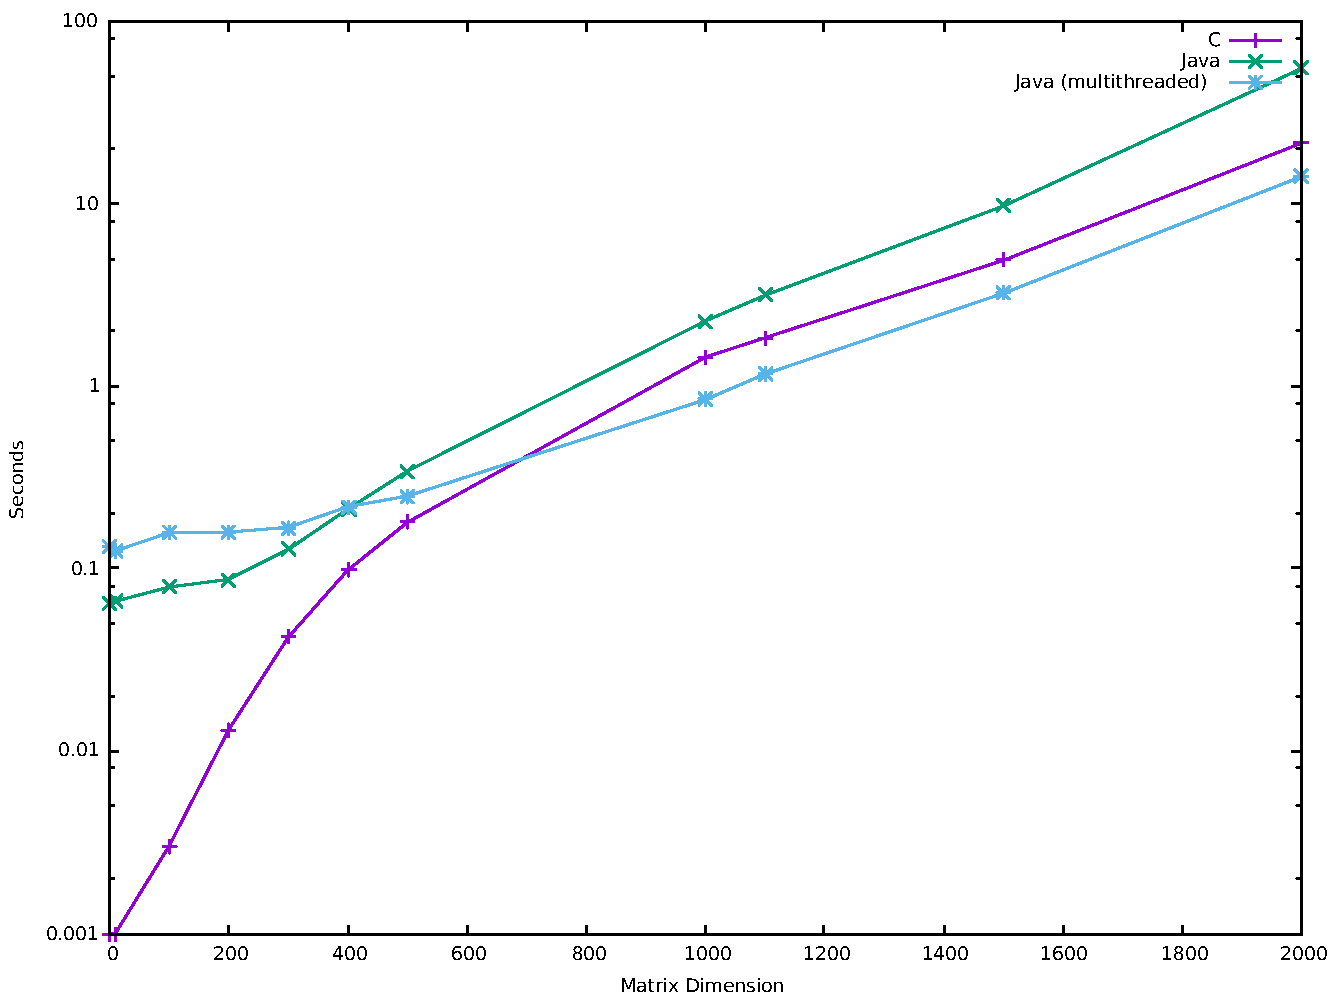
\includegraphics[width=\textwidth]{AppliedAlgorithmsMatrixMultiplicationPlots.pdf}
		\caption{Graphical presentation of the data. Note the logarithmic scale of the y-axis. As seen in the data, the Java-programs have a fairly high upstart penalty.}
		\label{fig:plots}
	\end{figure}

	\section{Conclusion}
	As it can be seen in the measurements, the C program outperforms the single threaded Java program in all the tested problem sizes. It can be discussed whether the 2D arrays in the single threaded Java implementation is fair against the C 1D arrays, but as the Java-runtime makes various optimizations on the bytecode I will not spend more time on optimizing the single threaded Java code.
	
	The Java Virtual Machine takes a small amount of time to start up, which is probably the reason that the Java programs are so much slower compared to the C program with small problem sizes. In the multi-threaded Java implementation, this situation is even worse because of the overhead of creating threads.

	Although the multi-threaded Java implementation is better than the single-threaded C implementation it can be seen from \autoref{fig:plots} that the computation time still grows polynomially in the problem size. This is easily seen as the y-axis is logarithmic, and the plot of the multi-threaded Java implementation seems linear.

% Appears to be instead of "it can be seen in the figure" - because the figure is finite.
% Or even better: In the range that we have observed.
% log-log: Will show the degree of the polynomial.

% Remember to run the experiments multiple times, to make it possible to account for a variance in jitter.

\end{document}
